\documentclass{beamer}

\usepackage{cite,doi}
\usepackage{amsmath,amssymb,amsfonts}
\usepackage{algorithm,algpseudocode}
\usepackage{stackengine,graphicx}
\usepackage{textcomp}
\usepackage{xcolor}
\usepackage{cleveref}
\usepackage{tikz}
\usetikzlibrary{3d}
\usetikzlibrary{patterns}
\usetikzlibrary{calc}
\usetikzlibrary{arrows}
\usetikzlibrary{matrix}
\usetikzlibrary{positioning}
\usetikzlibrary{decorations.pathreplacing}
\usepackage{mathtools}
\usepackage{subcaption}
\usepackage{import}
\usepackage{bm}
\usepackage[mathscr]{eucal}
\usepackage{amsbsy}
\usepackage[section]{placeins}
\usepackage{adjustbox}
\stackMath

\usepackage{../ourmacros}

\newcommand{\T}[1]{\boldsymbol{\mathscr{#1}}}


\newcommand{\hyper}{DC-HYDICE}
\newcommand{\image}{SIIM-ISIC}

\definecolor{wfugold}{rgb}{0.6196078,0.494117647,0.21960784}
\newcommand{\red}[1]{\textcolor{red}{#1}}
\newcommand{\blue}[1]{\textcolor{blue}{#1}}
\newcommand{\multiplycolor}{red}
\newcommand{\zero}{}
\newcommand{\cred}[1]{\textcolor{red}{#1}}
\newcommand{\cblue}[1]{\textcolor{blue}{#1}}
\newcommand{\cgold}[1]{\textcolor{wfugold}{#1}}
\newcommand{\email}[1]{\href{mailto:#1}{\texttt{#1}}}


\newlength\matfield
\newlength\tmplength
\def\matscale{1.}
\newcommand{\dimbox}[3]{%
  \setlength\matfield{\matscale\baselineskip}%
  \setbox0=\hbox{\vphantom{X}\smash{#3}}%
  \setlength{\tmplength}{#1\matfield-\ht0-\dp0}%
  \fboxrule=1pt\fboxsep=-\fboxrule\relax%
  \fbox{\makebox[#2\matfield]{\addstackgap[.5\tmplength]{\box0}}}%
}
\newcommand{\raiserows}[2]{%
   \setlength\matfield{\matscale\baselineskip}%
   \raisebox{#1\matfield}{#2}%
}
\newcommand{\matbox}[5]{
  \stackunder{\dimbox{#1}{#2}{$#5$}}{\scriptstyle(#3\times #4)}%
}


\title{Parallel Algorithms for Low-Rank Approximations of Matrices and Tensors}

\author{
    Lawton Manning
}

\usetheme{Warsaw}
\usecolortheme[named=wfugold]{structure}
%Madrid
%\usecolortheme{dolphin}
%\useinnertheme{rounded}
%\usefonttheme{serif}
\setbeamertemplate{navigation symbols}{} % gets rid of navigation bars
\setbeamertemplate{footline}
{
  \hbox{%
  \begin{beamercolorbox}[wd=.33\paperwidth,ht=2.25ex,dp=1ex,left]{author in head/foot}%
    \usebeamerfont{author in head/foot}
    Manning
  \end{beamercolorbox}%
  \begin{beamercolorbox}[wd=.34\paperwidth,ht=2.25ex,dp=1ex,center]{title in head/foot}%
    \usebeamerfont{title in head/foot}
    Thesis Proposal
  \end{beamercolorbox}%
  \begin{beamercolorbox}[wd=.33\paperwidth,ht=2.25ex,dp=1ex,right]{date in head/foot}%
    \usebeamerfont{date in head/foot}
    \insertframenumber{} \hspace*{2ex} 
  \end{beamercolorbox}}%
}


\begin{document}

\frame{\titlepage}

\begin{frame}{Introduction}
    \begin{itemize}
        \item Parallel Hierarchical Clustering using Rank-Two Nonnegative Matrix Factorization
        \item Tensor Train Rounding Using Gram Matrices
    \end{itemize}
\end{frame}

\begin{frame}{Nonnegative Matrix Factorization (NMF)}
    \begin{adjustbox}{max totalsize={.4\textwidth}{.5\textheight},center}
    \import{..}{fig/nmf}
    \end{adjustbox}
    \begin{itemize}
        \item approximate $\M{A}$ (features $\times$ samples) into $\M{W}$ (features $\times k$) and $\M{H}$ (samples $\times k$)
        \item nonnegativity gives interpretability of $\M{W}$ and $\M{H}$ as clusters and cluster membership, respectively
        \item applications
            \begin{itemize}
                \item text document clustering using bag of words or TF-IDF matrices
                \item hyperspectral image segmentation
            \end{itemize}
    \end{itemize}
\end{frame}

\begin{frame}{Hierarchical NMF}
    \begin{itemize}
        \item repeatedly use NMF with $k = 2$ to create a hierarchical tree of clusters
        \item application: hyperspectral imaging
    \end{itemize}
    \begin{adjustbox}{max totalsize={.7\textwidth}{.6\textheight},center}
    \import{..}{fig/dc}
    \end{adjustbox}
\end{frame}

\begin{frame}{Solving NMF}
    \begin{itemize}
        \item constrained optimization: $$\min_{\M{W},\M{H}\geq \M{0}} \|\M{A} - \M{W}\M{H}^\Tra\|_2$$
        \item Alternating Nonnegatively Constrained Least Squares (ANLS)
        \begin{itemize}
            \item fix $\M{H}$ and solve the NLS for $\M{W}$ exactly
            \item alternate and repeat until convergence
        \end{itemize}

        \item Block Principal Pivoting (BPP)
        \begin{itemize}
            \item solve unconstrained system
            \item $\M{W}^\Tra\M{W}$ and $\M{W}^\Tra\M{A}$ for $\M{H}$ and likewise for $\M{W}$
            \item account for negative solutions with active-set method (quadratic in $k$)
        \end{itemize}
    \end{itemize}
\end{frame}

\begin{frame}{Rank-2 NMF (R2NMF) NLS}
    \begin{itemize}
        \item when $k = 2$, the NLS can be solved quickly as the size of the active set is 4
        \item Active Sets for R2NMF (row by row)
        \begin{itemize}
            \item both columns nonnegative
            \item only left column nonnegative
            \item only right column nonnegative
            \item both columns negative
        \end{itemize}
    \end{itemize}
\end{frame}

\begin{frame}{Parallel R2NMF}
    \begin{itemize}
        \item distribute rows of $\M{A}$ onto separate processors
        \item distribute rows of $\M{W}$ and $\M{H}$ evenly
        \begin{itemize}
            \item $\M{W}^\Tra\M{A}$ and $\M{W}^\Tra\M{W}$ for $\M{H}$
            \item $(\M{A}\M{H})^\Tra$ and $\M{H}^\Tra\M{H}$ for $\M{W}$
        \end{itemize}
    \end{itemize}
        \import{..}{fig/r2nmf}
\end{frame}

\begin{frame}{Splitting with R2NMF}
    \begin{itemize}
        \item use columns of $\M{H}^\Tra$ to partition the columns of $\M{A}$ into clusters
        \item assign the cluster columns into two submatrices
        \item assign the corresponding columns of $\M{W}$ to the submatrices
        \item repeat NMF and split on submatrices
    \end{itemize}
    \begin{adjustbox}{max totalsize={.7\textwidth}{.6\textheight},center}
        \import{..}{fig/split}
    \end{adjustbox}
\end{frame}

\begin{frame}{HierNMF}
    \begin{itemize}
        \item split root node into two children with R2NMF
        \item power iteration $S\left(\cal N\right) = \sigma_1^2\left(\cal L\right) +
        \sigma_1^2\left(\cal R\right) -
        \sigma_1^2\left(\cal N\right)$
        \begin{itemize}
            \item heuristic for choosing next node to split
            \item requires node to have precomputed children
        \end{itemize}
        \item repeat until maximum number of nodes is reached or all child matrices are rank-1
    \end{itemize}
    \begin{adjustbox}{max totalsize={.7\textwidth}{.6\textheight},center}
        \import{..}{fig/tree}
    \end{adjustbox}
\end{frame}

\begin{frame}{Data Sets}
    \begin{itemize}
        \item DC-HYDICE
        \begin{itemize}
            \item Hyperspectral Digital Imagery Collection Experiment (HYDICE) of the National Mall in Washington, DC
        \end{itemize}
        \item SIIM-ISIC
        \begin{itemize}
            \item Society for Imaging Informatics in Medicine - International Skin Imaging Colloboration image classification of melanoma images
        \end{itemize}
        \item Synthetic Image classification
        \begin{itemize}
            \item smaller image classification dataset which has the same aspect ratio as SIIM-ISIC but small enough to fit in memory on one machine
        \end{itemize}
    \end{itemize}
\end{frame}

\begin{frame}{R2NMF Strong Scaling}
    \centering
    \begin{columns}
        \begin{column}{0.5\textwidth}
            \begin{figure}
            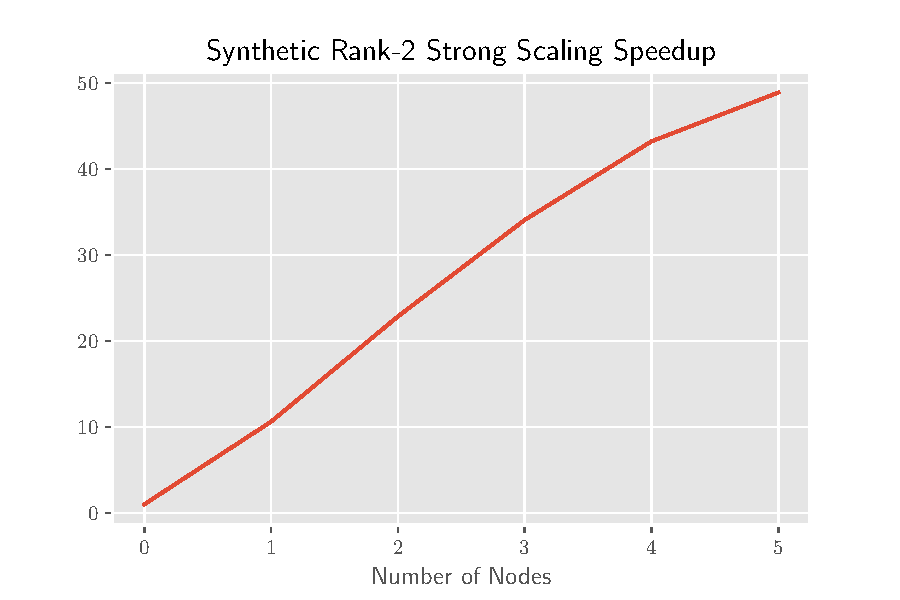
\includegraphics[width=\textwidth]{../plots/synthetic_rank2_speedup.pdf}
            \caption{Synthetic  Data}
            \end{figure}
        \end{column}
        \begin{column}{0.5\textwidth}
            \begin{figure}
            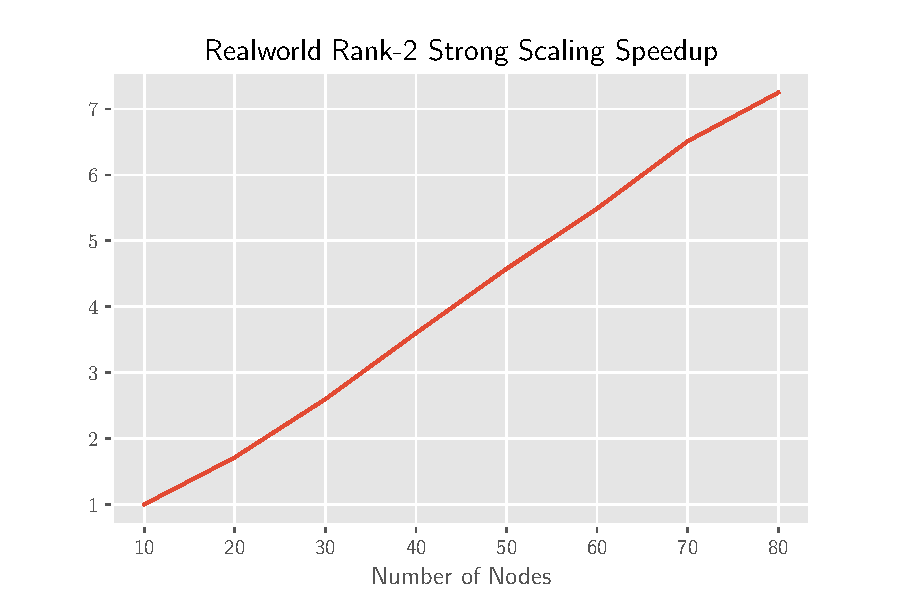
\includegraphics[width=\textwidth]{../plots/realworld_rank2_speedup.pdf}
            \caption{\image{} Data}
            \end{figure}
        \end{column}
    \end{columns}
\end{frame}

\begin{frame}{R2NMF Scaling Time Breakdowns}
    \centering
    \begin{columns}
        \begin{column}{0.5\textwidth}
            \begin{figure}
            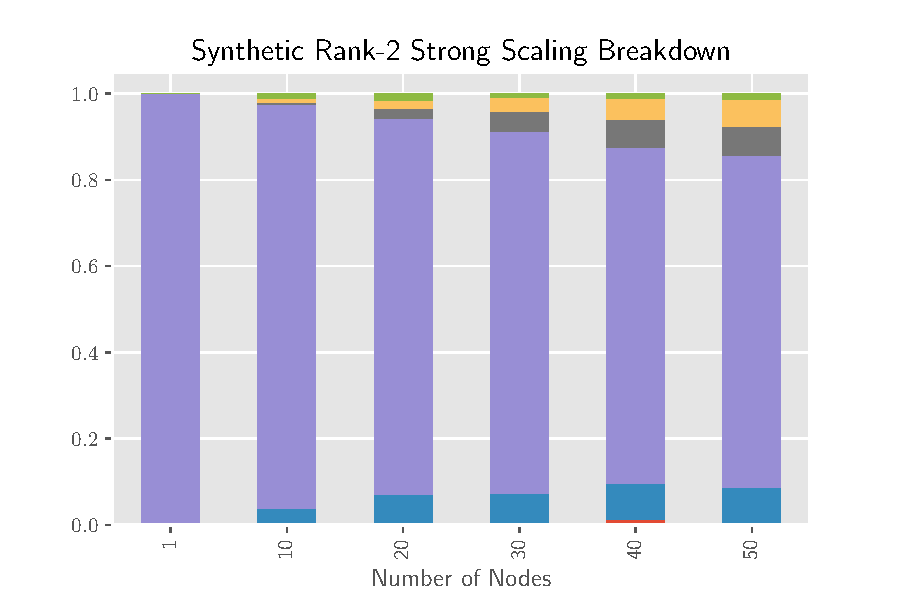
\includegraphics[width=\textwidth]{../plots/synthetic_rank2_strongscaling.pdf}
            \caption{Synthetic  Data}
            \end{figure}
        \end{column}
        \begin{column}{0.5\textwidth}
            \begin{figure}
            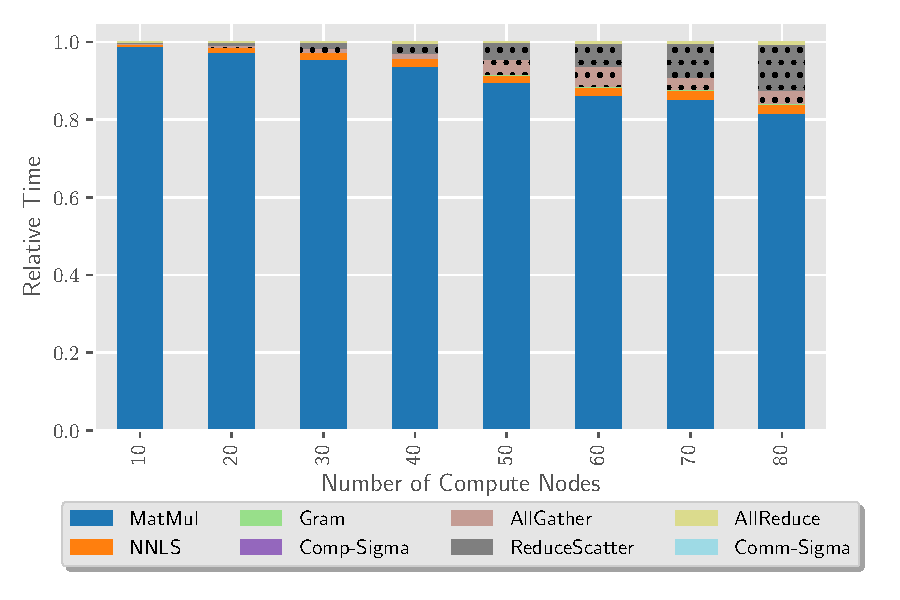
\includegraphics[width=\textwidth]{../plots/realworld_rank2_strongscaling.pdf}
            \caption{\image{} Data}
            \end{figure}
        \end{column}
    \end{columns}
\end{frame}

\begin{frame}{HierNMF Strong Scaling}
    \centering
    \begin{columns}
        \begin{column}{0.5\textwidth}
            \begin{figure}
            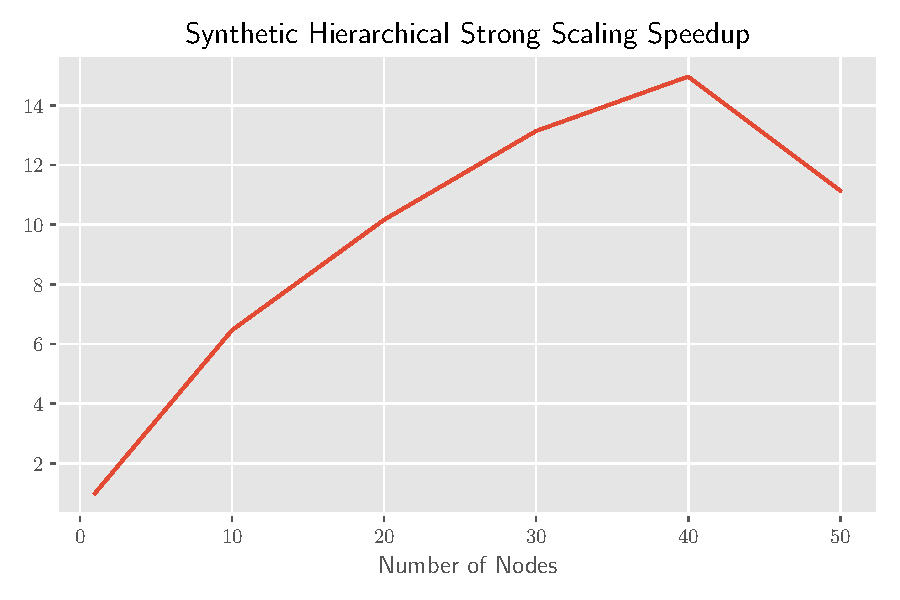
\includegraphics[width=\textwidth]{../plots/synthetic_hierarchical_speedup.pdf}
            \caption{Synthetic  Data}
            \end{figure}
        \end{column}
        \begin{column}{0.5\textwidth}
            \begin{figure}
            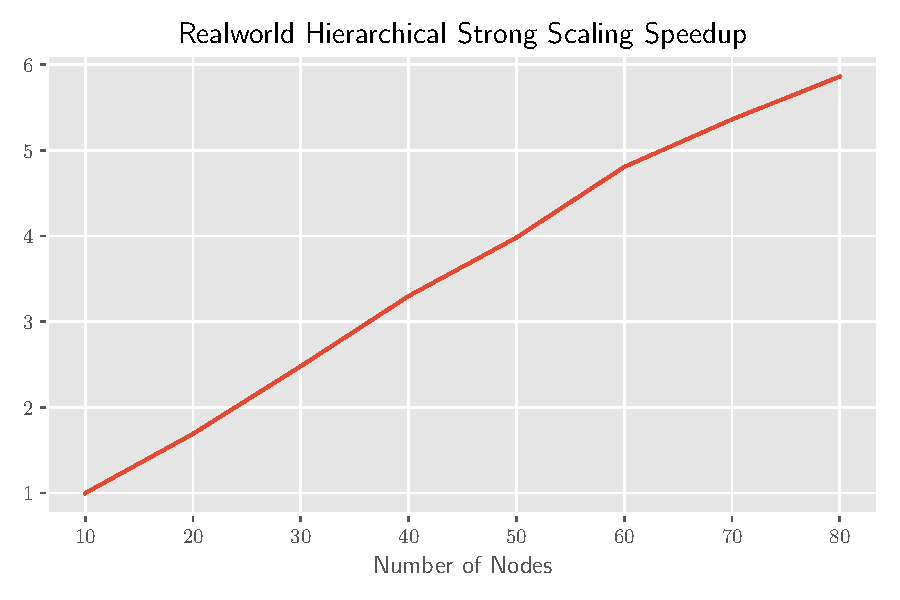
\includegraphics[width=\textwidth]{../plots/realworld_hierarchical_speedup.pdf}
            \caption{\image{} Data}
            \end{figure}
        \end{column}
    \end{columns}
\end{frame}

\begin{frame}{HierNMF Scaling Time Breakdowns}
    \centering
    \begin{columns}
        \begin{column}{0.5\textwidth}
            \begin{figure}
            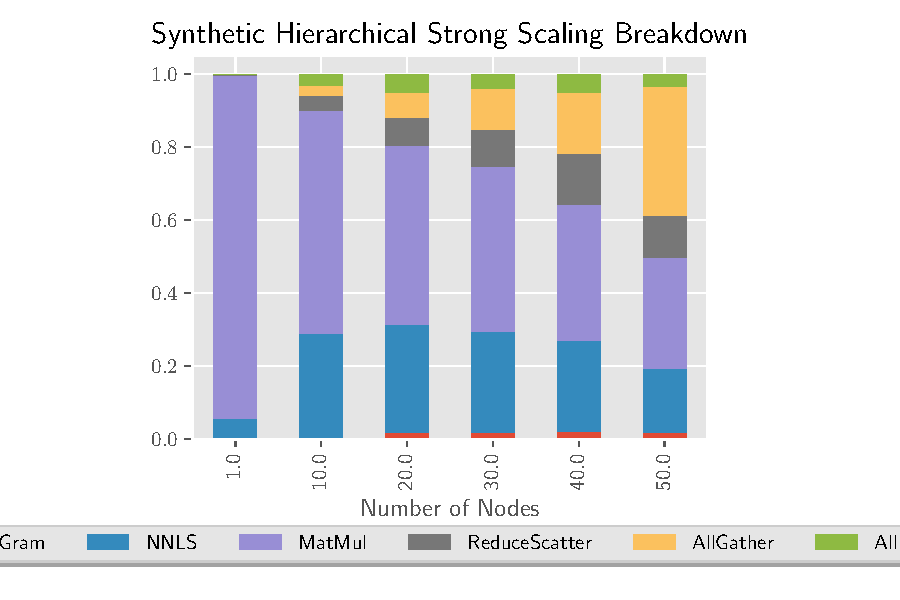
\includegraphics[width=\textwidth]{../plots/synthetic_hier_strongscaling.pdf}
            \caption{Synthetic  Data}
            \end{figure}
        \end{column}
        \begin{column}{0.5\textwidth}
            \begin{figure}
            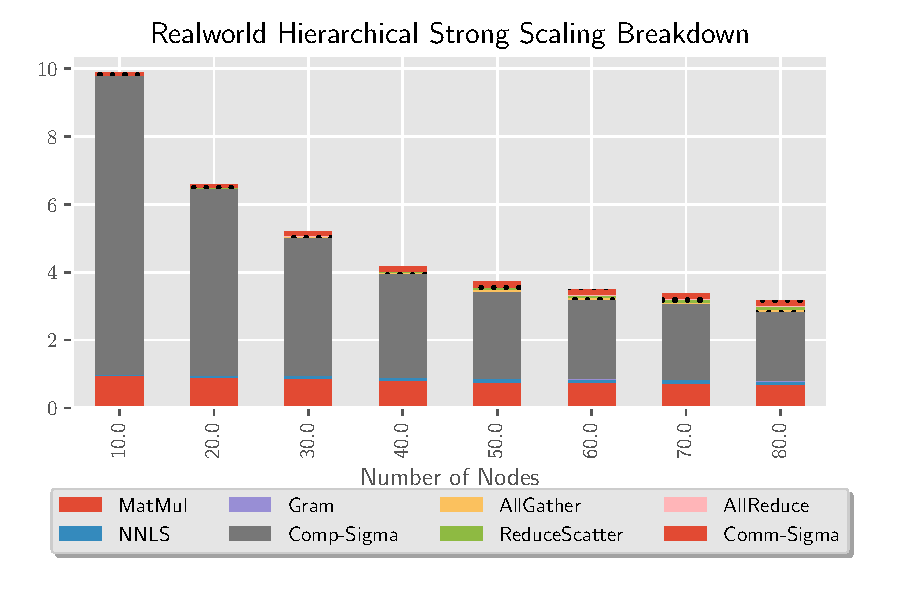
\includegraphics[width=\textwidth]{../plots/realworld_hier_strongscaling.pdf}
            \caption{\image{} Data}
            \end{figure}
        \end{column}
    \end{columns}
\end{frame}

\begin{frame}{Tree Level Times on Synthetic Data}
    \centering
    \begin{columns}
        \begin{column}{0.5\textwidth}
            \begin{figure}
            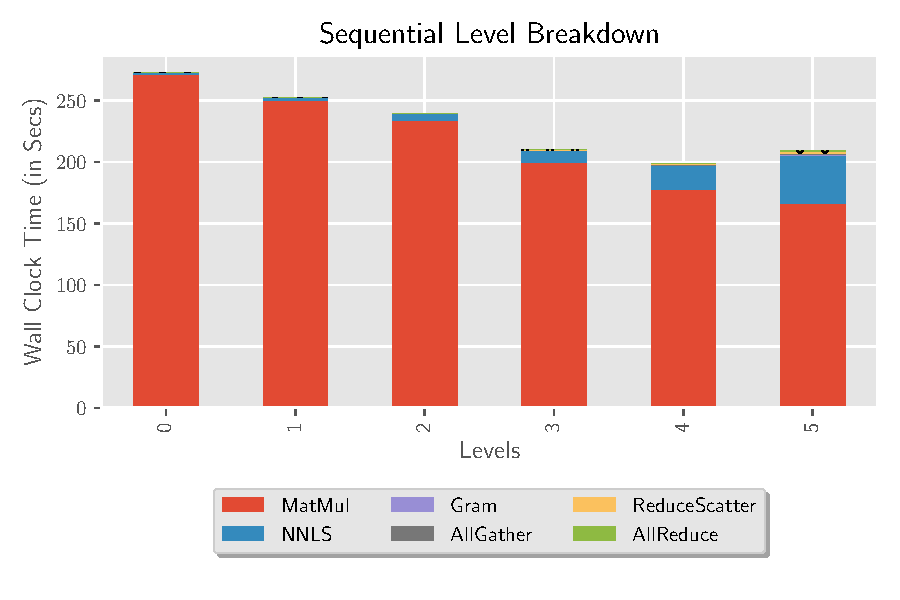
\includegraphics[width=\textwidth]{../plots/synthetic_sequential_level_breakdown.pdf}
            \caption{1 Compute Node}
            \end{figure}
        \end{column}
        \begin{column}{0.5\textwidth}
            \begin{figure}
            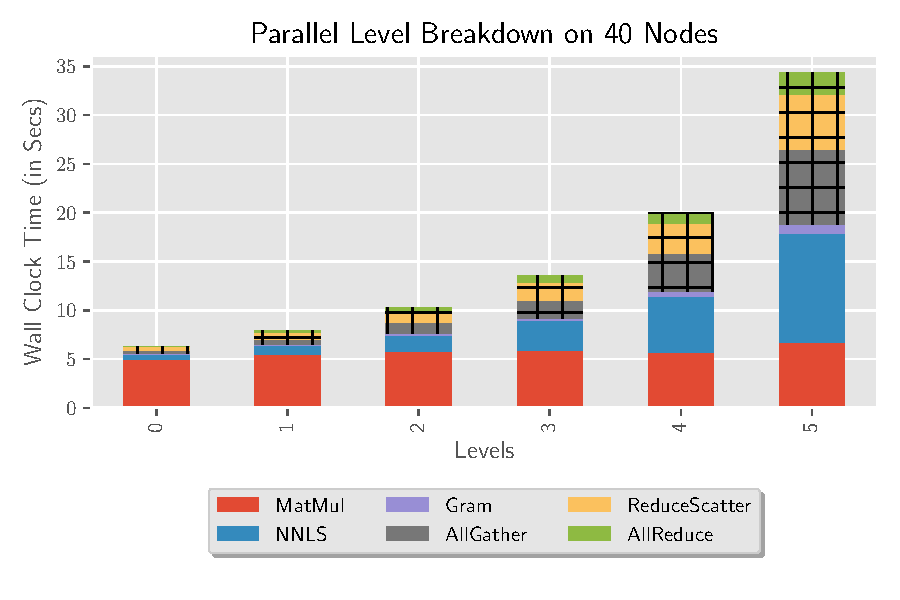
\includegraphics[width=\textwidth]{../plots/synthetic_parallel_level_breakdown.pdf}
            \caption{40 Compute Nodes}
            \end{figure}
        \end{column}
    \end{columns}
\end{frame}

\begin{frame}{Rank Scaling for Hierarchical and Flat NMF}
    \centering
    \begin{columns}
        \begin{column}{0.5\textwidth}
            \begin{figure}
            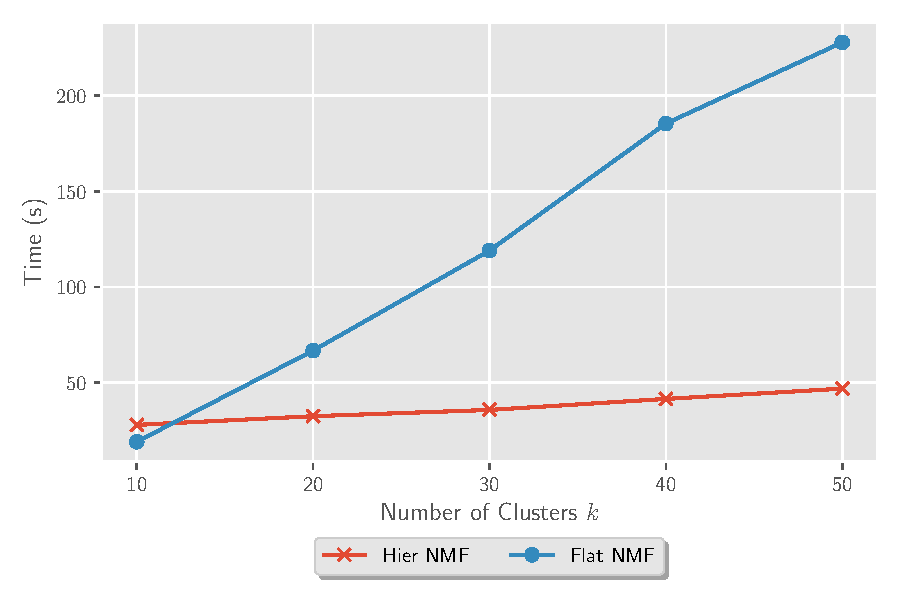
\includegraphics[width=\textwidth]{../plots/dc_rankscaling.pdf}
            \caption{\hyper{}  Data}
            \end{figure}
        \end{column}
        \begin{column}{0.5\textwidth}
            \begin{figure}
            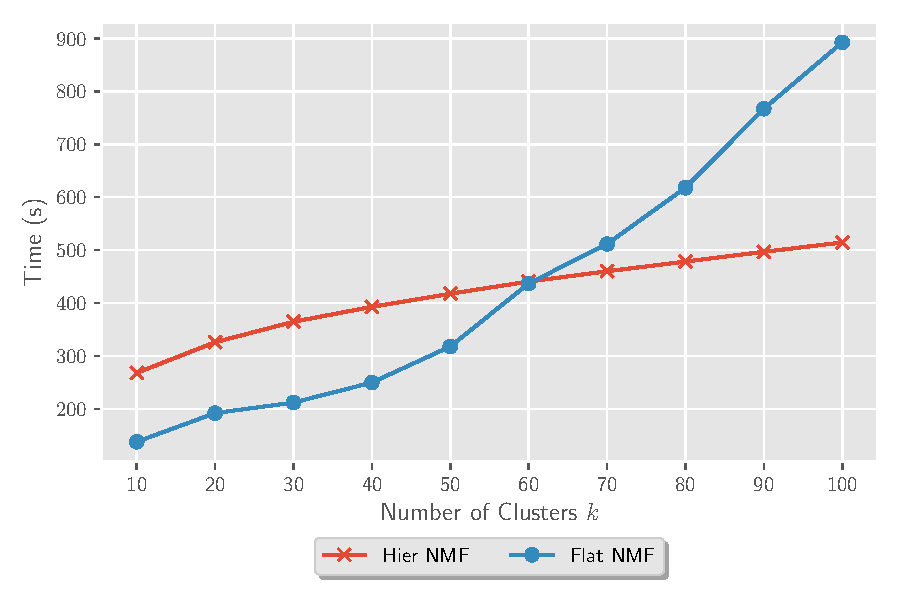
\includegraphics[width=\textwidth]{../plots/synthetic_rankscaling.pdf}
            \caption{Synthetic Data}
            \end{figure}
        \end{column}
    \end{columns}
\end{frame}



\begin{frame}
    \frametitle{Author Contact Information}
    
    For questions, please contact
    \begin{itemize}
        \item Lawton Manning: \email{mannlg15@wfu.edu}
        \item Grey Ballard: \email{ballard@wfu.edu}
        \item Ramakrishnan Kannan: \email{kannanr@ornl.gov}
        \item Haesun Park: \email{hpark@cc.gatech.edu}
    \end{itemize}
    
\end{frame}
    

\end{document}